%% chapter10_slides.tex
%% Beamer slides for Chapter 10: Bayesian Neural Network Inference of Motor
%% Insurance Claims
%% Bayesian Machine Learning in Quantitative Finance: Theory and Practical
%% Applications (Mongwe, Mbuvha & Marwala, Springer, 2025)
%% Reader-friendly style: complete sentences, symbol explanations, worked examples
%% Compiled with: pdflatex -interaction=nonstopmode chapter10_slides.tex  (twice)
\documentclass[aspectratio=169,10pt]{beamer}

\usetheme{Madrid}
\usecolortheme{seahorse}
\usefonttheme{professionalfonts}

%% ── Packages ──────────────────────────────────────────────────────────────
\usepackage{amsmath,amssymb,amsfonts}
\usepackage{mathtools}
\usepackage{graphicx}
\usepackage{booktabs}
\usepackage{xcolor}
\usepackage{listings}

\graphicspath{{figures/}}

%% ── Python listing style ─────────────────────────────────────────────────
\lstdefinestyle{pycode}{
  language=Python,
  basicstyle=\ttfamily\scriptsize,
  numbers=left,
  numberstyle=\tiny\color{gray},
  frame=single,
  backgroundcolor=\color{gray!7},
  keywordstyle=\color{blue!70!black}\bfseries,
  commentstyle=\color{green!50!black}\itshape,
  stringstyle=\color{orange!80!black},
  showstringspaces=false,
  breaklines=true,
  tabsize=2,
  xleftmargin=1.5em,
  framexleftmargin=1.5em,
  aboveskip=4pt,
  belowskip=4pt,
}
\lstset{style=pycode}

%% ── Metadata ─────────────────────────────────────────────────────────────
\title[Bayesian ML in QF -- Ch.10]{Bayesian Machine Learning in Quantitative Finance}
\subtitle{Chapter 10: Bayesian Neural Networks for Motor Insurance Claims}
\author{Based on Mongwe, Mbuvha \& Marwala}
\institute{Springer, 2025}
\date{}

\setbeamertemplate{footline}[frame number]
\setbeamertemplate{navigation symbols}{}

%% Helpful macros
\newcommand{\bw}{\mathbf{w}}
\newcommand{\bx}{\mathbf{x}}

%% ══════════════════════════════════════════════════════════════════════════
\begin{document}

%% ── Title frame ──────────────────────────────────────────────────────────
\begin{frame}
  \titlepage
\end{frame}

%% ── Outline ──────────────────────────────────────────────────────────────
\begin{frame}{Chapter Overview}
  \tableofcontents
\end{frame}

\AtBeginSection[]{\begin{frame}{Outline}\tableofcontents[currentsection]\end{frame}}

%% ══════════════════════════════════════════════════════════════════════════
\section{10.1 Introduction}
%% ══════════════════════════════════════════════════════════════════════════

\begin{frame}[allowframebreaks]{10.1 Introduction: Motor Insurance and the Claim Prediction Problem}

Insurance is a form of risk management: a policyholder pays a premium so that,
if something bad happens, the insurer covers the loss. \textbf{Motor insurance}
is the subset of general (non-life) insurance concerned with vehicles ---
comprehensive cover typically includes theft, accidents, and third-party
liability. Because motor insurance generates enormous amounts of policy and
claims data, it is a natural target for machine learning.

  \begin{block}{Why Claim Prediction Matters}
    For every policy, an insurer wants to know: \emph{how likely is this
    policyholder to file a claim this year?}  Answering this well matters for
    two reasons: (1) \textbf{pricing} -- premiums should reflect risk, and
    (2) \textbf{fraud detection} -- unusual claim patterns can be flagged.
    Traditionally, insurers used \textbf{Generalised Linear Models (GLMs)}
    that assume a linear relationship between policy features and claim
    frequency/severity, and assume claim frequency and severity are
    independent. Real claims data rarely obey either assumption exactly.
  \end{block}

  \begin{block}{The Shift Toward Machine Learning}
    As computing power and data volumes have grown, machine learning models
    -- gradient-boosted trees and neural networks in particular -- have
    increasingly been used to model claim frequency and severity, since they
    can capture non-linear relationships and interactions between features
    that a GLM would miss. Neural networks in particular have repeatedly been
    found to be strong predictors of claim size and claim occurrence in the
    actuarial literature.
  \end{block}

  \begin{alertblock}{The Gap This Chapter Fills}
    Almost all of this machine learning literature produces a single
    \textbf{point prediction}: ``this policy has an 8\% chance of a claim,''
    full stop. Very little attention has been paid to \textbf{Bayesian}
    approaches, which instead return a \emph{whole distribution} over that
    probability -- telling you not just the estimate, but how confident the
    model is in that estimate. This chapter fills that gap: it uses
    \textbf{Bayesian Neural Networks (BNNs)} with \textbf{Automatic Relevance
    Determination (ARD)} priors to predict whether a motor insurance policy
    will generate a claim, trained via the \textbf{Laplace approximation}.
    The ARD prior has a second benefit: it lets us rank which input features
    matter most for the prediction.
  \end{alertblock}

  \framebreak

  \begin{block}{Two Uses of Bayesian Inference in this Chapter}
    \begin{itemize}
      \item \textbf{Parameter estimation}: given a fixed network architecture,
        find the plausible values (really, the full \emph{distribution} of
        plausible values) for its weights. This is usually done with sampling
        methods such as Markov chain Monte Carlo (MCMC).
      \item \textbf{Model selection}: compare \emph{different} architectures
        (e.g., a small network vs.\ a deep one) using the \textbf{Bayesian
        evidence} $P(D \mid H)$ -- the probability of the observed data $D$
        under model/architecture $H$, averaged over all possible weight
        settings. Higher evidence means the architecture explains the data
        better \emph{without} needing to fit held-out data first.
      \end{itemize}
    Evaluating the evidence exactly is hard for a model as complex as a
    neural network, so approximations are needed: Bayesian quadrature, nested
    sampling, and the \textbf{Laplace approximation} of MacKay (1992) are the
    three most established options. MCMC is guaranteed to converge to the
    true posterior eventually but is computationally expensive; this chapter
    instead uses the Laplace approximation, which is far cheaper and, as we
    will see, scales comfortably to networks with hundreds of parameters.
  \end{block}

  \begin{exampleblock}{Roadmap for This Chapter}
    \begin{itemize}
      \item \textbf{Sect.\ 10.2}: how a Bayesian neural network is set up
        (priors over weights, likelihood, posterior).
      \item \textbf{Sect.\ 10.3}: the Laplace approximation used to make that
        posterior tractable.
      \item \textbf{Sect.\ 10.4}: the real dataset (3000 Spanish motor
        policies) and the experimental setup.
      \item \textbf{Sect.\ 10.5--10.6}: results across six network
        architectures, and conclusions.
    \end{itemize}
  \end{exampleblock}

\end{frame}

%% ══════════════════════════════════════════════════════════════════════════
\section{10.2 Bayesian Neural Network Models}
%% ══════════════════════════════════════════════════════════════════════════

\begin{frame}[allowframebreaks]{10.2 What Is a Bayesian Neural Network? -- Plain-Language Intuition}

You already know an ordinary (non-Bayesian) feed-forward neural network:
data flows forward through layers of neurons, each layer computing a weighted
sum of its inputs followed by a non-linear activation, and training finds
\emph{one} set of weights that minimises a loss function. A \textbf{Bayesian
neural network (BNN)} changes only one thing conceptually, but that one
change has big consequences.

  \begin{alertblock}{The Core Idea, in One Sentence}
    Instead of committing to a single ``best'' set of weights, put a
    \textbf{prior probability distribution over every weight} in the network,
    and after seeing the training data, compute a \textbf{posterior
    distribution over the weights} instead of a single fixed value. Feeding
    an input through this whole distribution of weights (rather than one
    fixed network) gives you not just a point prediction, but a
    \emph{distribution of predictions} -- genuine, quantified uncertainty.
  \end{alertblock}

  \begin{block}{Why This Matters for Insurance Claims}
    If a model predicts ``12\% chance of a claim'' for two different
    policyholders, a Bayesian model can additionally tell you \emph{how sure}
    it is of that 12\% for each one. A policy that looks like thousands of
    others in the training data will get a narrow, confident distribution.
    A policy with an unusual combination of features (e.g., a very rare
    vehicle type) will get a wide, uncertain distribution -- even if the
    point estimate is the same 12\%. Knowing which is which matters directly
    for risk management and pricing decisions.
  \end{block}

  \framebreak

  \begin{block}{The Network Architecture (Eq.\ 10.1--10.2)}
    This chapter uses fully connected feed-forward networks. For a network
    with one hidden layer, the output and hidden-layer computations are:
    \[
      f_k(\bx) = b_k + \sum_j v_{jk}\, h_j(\bx),
      \qquad
      h_j(\bx) = \Psi\!\left(a_j + \sum_i w_{ij}\, x_i\right).
    \]
    \begin{itemize}
      \item $x_i$ is the $i$-th input feature (e.g.\ driver age, vehicle
        power); $h_j(\bx)$ is the activation of the $j$-th hidden neuron.
      \item $w_{ij}$ is the weight connecting input $i$ to hidden unit $j$;
        $a_j$ is that hidden unit's bias.
      \item $v_{jk}$ is the weight connecting hidden unit $j$ to output $k$
        (here $k=1$, a single output: the probability of a claim); $b_k$ is
        the output bias.
      \item $\Psi$ is the activation function providing the non-linearity;
        this chapter uses $\tanh$ throughout for every hidden layer.
    \end{itemize}
    In the \emph{ordinary} (non-Bayesian) network, $w_{ij}, a_j, v_{jk}, b_k$
    are all just numbers, fixed once training finishes. In a BNN, every one
    of these is instead treated as a random variable with its own
    distribution -- collect them all into one long vector $\bw$ (bold w),
    the full weight vector of the network.
  \end{block}

  \framebreak

  \begin{block}{Bayes' Theorem for Neural Network Weights (Eq.\ 10.3)}
    \[
      P(\bw \mid D, H) = \frac{P(D \mid \bw, H)\, P(\bw \mid H)}{P(D \mid H)}.
    \]
    \begin{itemize}
      \item $D$ is the training data (the observed policies and whether they
        claimed); $H$ denotes the model \emph{architecture} (how many
        layers, how many hidden units -- this chapter compares six choices
        of $H$).
      \item $P(\bw \mid H)$ is the \textbf{prior}: what we believe about
        plausible weight values \emph{before} seeing any data. It can be set
        individually per weight, or the same for every weight in the
        network.
      \item $P(D \mid \bw, H)$ is the \textbf{likelihood}: how probable the
        observed claims data is, for a given setting of the weights.
      \item $P(\bw \mid D, H)$ is the \textbf{posterior}: what we believe
        about the weights \emph{after} combining the prior with the evidence
        of the training data. This is the object we actually want, and its
        width represents our residual uncertainty.
      \item $P(D \mid H)$, the \textbf{evidence} (or marginal likelihood), is
        the normalising constant of Bayes' theorem here -- but it does double
        duty as a score for comparing entire architectures $H$, since it
        measures how well architecture $H$ explains $D$, averaged over every
        possible weight setting (not just the best one).
    \end{itemize}
  \end{block}

  \begin{alertblock}{Model Selection via the Bayes Factor (Eq.\ 10.4)}
    \[
      BF := \frac{P(D \mid H_1)}{P(D \mid H_2)} \cdot \frac{\pi(M_1)}{\pi(M_2)}
    \]
    where $\pi(M_i)$ is our prior belief that model $i$ is correct. If we have
    no reason to prefer one architecture over another a priori, $\pi(M_1) =
    \pi(M_2)$ and comparing models reduces to comparing their evidence
    values. $BF > 1$ favours $M_1$; $BF < 1$ favours $M_2$. Because the exact
    posterior $P(\bw \mid D, H)$ is analytically intractable for anything as
    complex as a neural network, it must be approximated numerically --
    which is exactly the job of the Laplace approximation in Sect.\ 10.3.
  \end{alertblock}

  \framebreak

  \begin{block}{The Six Architectures Compared in This Chapter}
    \begin{center}
    \begin{tabular}{lll}
      \toprule
      \textbf{Model} & \textbf{Architecture} & \textbf{Parameters} \\
      \midrule
      Model 1 & 1 hidden layer, 5 neurons   & 137 \\
      Model 2 & 1 hidden layer, 10 neurons  & 272 \\
      Model 3 & 1 hidden layer, 50 neurons  & 1352 \\
      Model 4 & 2 hidden layers, 5 neurons each  & 162 \\
      Model 5 & 2 hidden layers, 10 neurons each & 372 \\
      Model 6 & 3 hidden layers, 10 neurons each & 472 \\
      \bottomrule
    \end{tabular}
    \end{center}
    These six choices let the chapter compare \textbf{wide-and-shallow}
    (Models 1--3) against \textbf{narrower-and-deep} (Models 4--6)
    architectures, using the evidence framework of Sect.\ 10.3 to decide
    which is preferable -- rather than relying only on held-out accuracy.
  \end{block}

\end{frame}

\begin{frame}[fragile]{Python: A Small Feed-Forward Network (the ``H'' in $P(D\mid H)$)}

Before adding any Bayesian machinery, we need an ordinary point-estimate
network implementing Eqs.\ 10.1--10.2. This is exactly the object whose
weights we will later treat as random variables in Sect.\ 10.3 -- the
architecture ($H$) is fixed by the code below; the \emph{values} of
\texttt{w1}, \texttt{w2}, \texttt{b1}, \texttt{b2} are what become uncertain
in a BNN.

\begin{lstlisting}[caption={A tiny feed-forward net, matching Eqs. 10.1--10.2}]
import numpy as np

class TinyFeedForwardNet:
    """One hidden layer, tanh activation, matches Eq. 10.1-10.2."""
    def __init__(self, n_in, n_hidden, rng):
        # w_ij: input -> hidden weights;  a_j: hidden biases
        self.w = rng.normal(scale=0.5, size=(n_hidden, n_in))
        self.a = rng.normal(scale=0.5, size=n_hidden)
        # v_j: hidden -> output weights;  b: output bias
        self.v = rng.normal(scale=0.5, size=n_hidden)
        self.b = 0.0

    def forward(self, x):
        # h_j(x) = tanh(a_j + sum_i w_ij x_i)      -- Eq. 10.2
        h = np.tanh(self.a + self.w @ x)
        # f(x) = b + sum_j v_j h_j(x)               -- Eq. 10.1
        return self.b + self.v @ h

# H = "1 hidden layer, 5 neurons" is Model 1 in Table 10.1 (137 parameters
# once the input dimension of the motor-claims dataset is accounted for).
rng = np.random.default_rng(0)
net = TinyFeedForwardNet(n_in=27, n_hidden=5, rng=rng)
\end{lstlisting}

In an \emph{ordinary} network, \texttt{net.w}, \texttt{net.a}, \texttt{net.v},
\texttt{net.b} are single fixed arrays of numbers, updated by gradient
descent. A Bayesian neural network instead maintains a whole probability
distribution over each of these arrays -- Sect.\ 10.3 shows how the Laplace
approximation makes this practical.

\end{frame}

\begin{frame}{Illustration: Weights as Distributions, Not Numbers}

  \begin{center}
    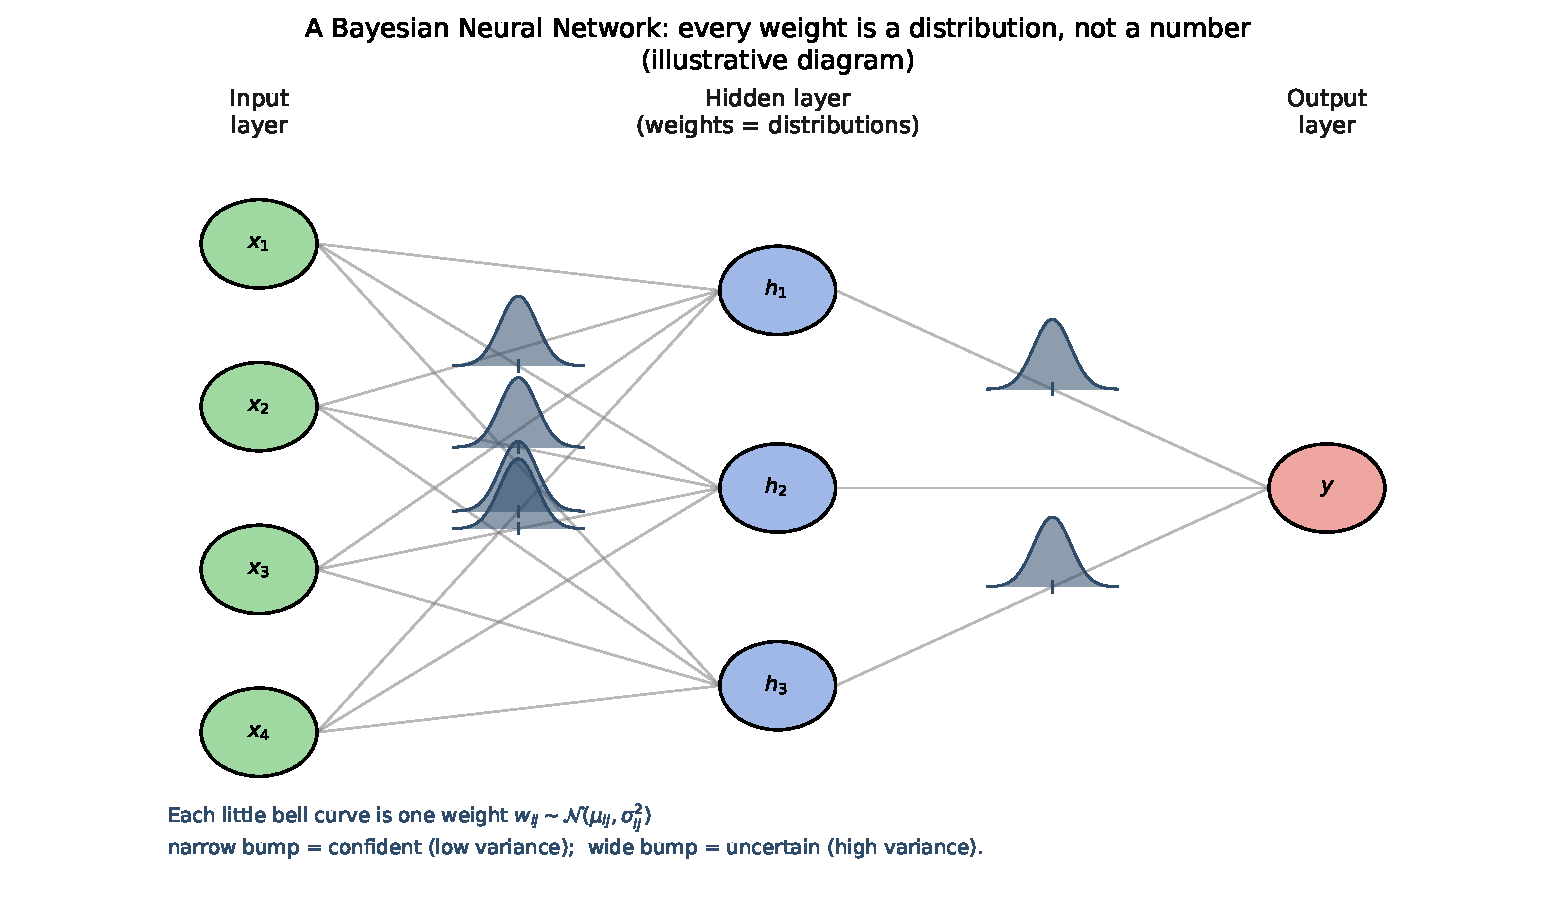
\includegraphics[width=0.92\linewidth]{fig_bnn_weight_uncertainty}
  \end{center}

  \begin{block}{Reading the Diagram}
    Every connection in an ordinary network carries one number, $w_{ij}$.
    In a Bayesian network, every connection instead carries a distribution
    $w_{ij} \sim \mathcal{N}(\mu_{ij}, \sigma_{ij}^2)$ (mean $\mu_{ij}$,
    variance $\sigma_{ij}^2$). A \textbf{narrow} bell curve means the
    network is confident about that particular weight; a \textbf{wide} bell
    curve means genuine uncertainty about it. Sect.\ 10.3 explains exactly
    how $\mu_{ij}$ and $\sigma_{ij}^2$ are obtained for every weight, all at
    once, via the Laplace approximation.
  \end{block}

\end{frame}

%% ══════════════════════════════════════════════════════════════════════════
\section{10.3 Laplace Approximation to Bayesian Neural Networks}
%% ══════════════════════════════════════════════════════════════════════════

\begin{frame}[allowframebreaks]{10.3 The Laplace Approximation -- Plain-Language Intuition}

We now have a posterior $P(\bw \mid D, H)$ that we want, but cannot compute
exactly. The \textbf{Laplace approximation (LA)} is the simplest practical
way to approximate it.

  \begin{alertblock}{The Core Idea, in One Sentence}
    First find the single best (\textbf{MAP}, maximum a posteriori) set of
    weights $\bw_{MP}$ via ordinary training (exactly as you would train any
    neural network, just with a regularisation term built in). Then
    approximate the messy true posterior \emph{around that one point} as a
    \textbf{Gaussian} bell curve, using how sharply curved the loss surface
    is at $\bw_{MP}$ -- the \textbf{Hessian} (matrix of second derivatives)
    -- to set the width of that Gaussian. Sharp curvature (a narrow, steep
    valley) means a confident, narrow posterior; flat curvature (a wide,
    shallow valley) means an uncertain, wide posterior.
  \end{alertblock}

  \begin{block}{Why a Gaussian Centered at the Mode?}
    MacKay (1995a) proposed exactly this recipe for Bayesian neural
    networks. The key practical advantage: $\bw_{MP}$ can be obtained with
    completely standard MAP training of the network (an ordinary training
    loop with weight decay), and modern second-order optimisation tools make
    the required curvature (Hessian) estimates cheap to obtain even for
    networks with hundreds of parameters. This means the Laplace
    approximation can be bolted onto an \emph{already-trained} deep network,
    turning point predictions into distributions of predictions with very
    little extra engineering effort.
  \end{block}

  \framebreak

  \begin{block}{Setting Up the Exact Posterior (Eq.\ 10.5--10.6)}
    Assume the prior on the weights is Gaussian with mean zero and precision
    $\alpha$ (inverse variance), and let $\beta$ be the precision of the
    data-noise term. Then the (still-exact, but intractable) posterior is:
    \[
      P(\bw \mid \alpha, \beta, D, H) = \frac{1}{Z_M(\alpha,\beta)}
        \exp\big(-(\alpha E_{\bw} + \beta E_D)\big)
      = \frac{1}{Z_M(\alpha,\beta)} \exp(-M(\bw))
    \]
    where $M(\bw) := \alpha E_{\bw} + \beta E_D$.
    \begin{itemize}
      \item $E_{\bw} = \tfrac{1}{2}\lVert \bw \rVert^2$ is the \textbf{prior
        kernel}: a penalty growing with the size of the weights (this is
        exactly an $L_2$ / weight-decay penalty).
      \item $E_D$ is the \textbf{likelihood kernel}: the data-misfit term
        (e.g.\ sum-of-squared errors for regression, or cross-entropy for
        the claim/no-claim classification task used later in this chapter).
      \item $\alpha E_{\bw} + \beta E_D = M(\bw)$ is exactly the ordinary,
        \emph{regularised training loss} of the network. In other words:
        minimising the familiar training loss \emph{is} finding the mode of
        this Bayesian posterior.
      \item $Z_M(\alpha,\beta)$ is just a normalising constant so that the
        posterior integrates to one.
    \end{itemize}
  \end{block}

  \framebreak

  \begin{block}{The Gaussian (Laplace) Approximation Itself (Eq.\ 10.7--10.8)}
    MacKay's approximation performs a second-order Taylor expansion of the
    posterior around its mode $\bw_{MP}$:
    \[
      P(\bw \mid \alpha,\beta,D,H) \approx \frac{1}{Z_M'(\alpha,\beta)}
        \exp\left(-M(\bw) - \tfrac{1}{2} W(\alpha,\beta)\right),
      \qquad
      W(\alpha,\beta) = (\bw - \bw_{MP})^\top \mathbf{A} (\bw - \bw_{MP}).
    \]
    \begin{itemize}
      \item $\bw_{MP}$ is the \textbf{mode of the posterior} -- the MAP
        estimate, exactly what an ordinary (regularised) training run
        converges to.
      \item $\mathbf{A}$ is the matrix of \textbf{second derivatives of the
        negative log posterior} $M(\bw)$, evaluated at $\bw_{MP}$: this is
        the \textbf{Hessian}. It has one row/column per network parameter,
        so for a network with $g$ parameters, $\mathbf{A}$ is $g \times g$.
      \item $W(\alpha,\beta)$ is a quadratic form measuring how far a
        candidate $\bw$ is from the mode, \emph{weighted} by the curvature
        $\mathbf{A}$ in every direction.
    \end{itemize}
  \end{block}

  \begin{block}{The Normalising Constant Becomes Tractable (Eq.\ 10.9--10.10)}
    \[
      Z_M'(\alpha,\beta) = \int \exp\left(-M(\bw) -\tfrac{1}{2}(\bw-\bw_{MP})^\top
        \mathbf{A}(\bw-\bw_{MP})\right) d\bw
      = \exp(-M(\bw))\,(2\pi)^{-g/2}\,\det(\mathbf{A})^{-\frac{1}{2}}
    \]
    Here $g$ is the number of parameters in the network, and $\det(\mathbf{A})$
    is the determinant of the Hessian. This is precisely the normalising
    constant of a multivariate Gaussian -- confirming that the Laplace
    approximation is exactly $\bw \mid D \sim \mathcal{N}(\bw_{MP}, \mathbf{A}^{-1})$.
    Because this expression is now closed-form, both the evidence $P(D\mid H)$
    \emph{and} the optimal prior/noise precisions $\alpha,\beta$ (found by
    alternating gradient descent on the weights with evidence maximisation
    over $\alpha,\beta$) become computationally cheap to evaluate. This
    chapter uses the \textbf{Laplace} package in Python (Daxberger et al.,
    2021) to do exactly this.
  \end{block}

  \framebreak

  \begin{block}{The Laplace Approximation, Step by Step}
    \begin{enumerate}
      \item \textbf{Find the MAP estimate.} Train the network as usual,
        minimising $M(\bw) = \alpha E_{\bw} + \beta E_D$ (an ordinary loss
        plus a weight-decay penalty). The result is $\bw_{MP}$, a single
        best set of weights -- exactly what you would get from standard
        (non-Bayesian) training.
      \item \textbf{Compute (or approximate) the Hessian.} Evaluate
        $\mathbf{A} = \nabla^2_{\bw} M(\bw)\big|_{\bw = \bw_{MP}}$, the
        matrix of second derivatives of the negative log posterior at the
        MAP estimate. This measures how sharply the loss curves in every
        direction of weight space around $\bw_{MP}$.
      \item \textbf{Set the posterior covariance to the inverse Hessian.}
        Approximate $P(\bw \mid D, H) \approx \mathcal{N}(\bw_{MP},
        \mathbf{A}^{-1})$. Directions of high curvature (large entries of
        $\mathbf{A}$) get small posterior variance (confident); directions
        of low curvature (small entries of $\mathbf{A}$) get large posterior
        variance (uncertain).
      \item \textbf{Sample or propagate uncertainty through the network.}
        To get predictive uncertainty for a new input $\bx^*$, either (a)
        draw many weight samples $\bw^{(s)} \sim \mathcal{N}(\bw_{MP},
        \mathbf{A}^{-1})$ and run the network forward for each one, building
        up a distribution of predictions, or (b) linearise the network
        output around $\bw_{MP}$ and propagate the Gaussian directly (the
        ``delta method''): $\mathrm{Var}[f(\bx^*)] \approx
        \mathbf{J}(\bx^*)\, \mathbf{A}^{-1}\, \mathbf{J}(\bx^*)^\top$, where
        $\mathbf{J}(\bx^*)$ is the gradient of the network output with
        respect to $\bw$ at $\bx^*$.
    \end{enumerate}
  \end{block}

  \framebreak

  \begin{exampleblock}{Hand-Worked Numeric Example: A Single Scalar Weight}
    Consider the simplest possible case: a network with just \textbf{one}
    weight $\theta$ (so $g=1$ and the Hessian is just a single number, the
    ordinary scalar second derivative), predicting $\hat{y} = \theta x$ for
    one training example $x=1$, $y=3$. Take prior precision $\alpha=1$ and
    noise precision $\beta=1$, with $E_{\theta} = \tfrac{1}{2}\theta^2$ and
    $E_D = \tfrac{1}{2}(y - \theta x)^2$:
    \[
      M(\theta) = \tfrac{1}{2}\theta^2 + \tfrac{1}{2}(3-\theta)^2.
    \]

    \medskip
    \textbf{Step 1 (find the MAP):} $\dfrac{dM}{d\theta} = \theta - (3-\theta)
      = 2\theta - 3 = 0 \implies \theta_{MP} = 1.5$.

    \medskip
    \textbf{Step 2 (the ``Hessian,'' here a scalar second derivative):}
    $\dfrac{d^2 M}{d\theta^2} = 2$, so $A = 2$. This curvature does not
    depend on $\theta$ here because $M$ is an exact quadratic (a straight
    line has constant curvature) -- so in this special case the Laplace
    approximation is not an approximation at all, it is \emph{exact}.

    \medskip
    \textbf{Step 3 (posterior variance = inverse Hessian):}
    $\sigma^2 = 1/A = 0.5$.

    \medskip
    \textbf{Result:} $\theta \mid D \sim \mathcal{N}(1.5,\ 0.5)$ exactly.
    A confident model (informative data, sharp curvature) would give a
    larger $A$ and hence a smaller $\sigma^2$; a single noisy or ambiguous
    data point, as here, leaves meaningful residual uncertainty.
  \end{exampleblock}

  \begin{block}{What Happens with a Genuinely Non-Linear (Non-Quadratic) Loss?}
    Real neural networks are non-linear, so $M(\bw)$ is generally \emph{not}
    an exact quadratic bowl -- the true posterior can be skewed or
    multi-modal. The figure below shows a one-parameter toy case with a
    quartic correction term, $M(\theta) = \tfrac{1}{2}(\theta-1)^2 +
    0.08(\theta-1)^4$, illustrating that the Laplace Gaussian (matched to the
    curvature exactly at the mode) tracks the true posterior closely near
    the mode but increasingly departs from it in the tails -- exactly the
    approximation error that has been reported for Laplace approximations of
    genuinely multi-modal neural network posteriors (Mbuvha et al., 2017).
  \end{block}

\end{frame}

\begin{frame}{Illustration: Laplace Approximation of a Non-Gaussian Posterior}

  \begin{center}
    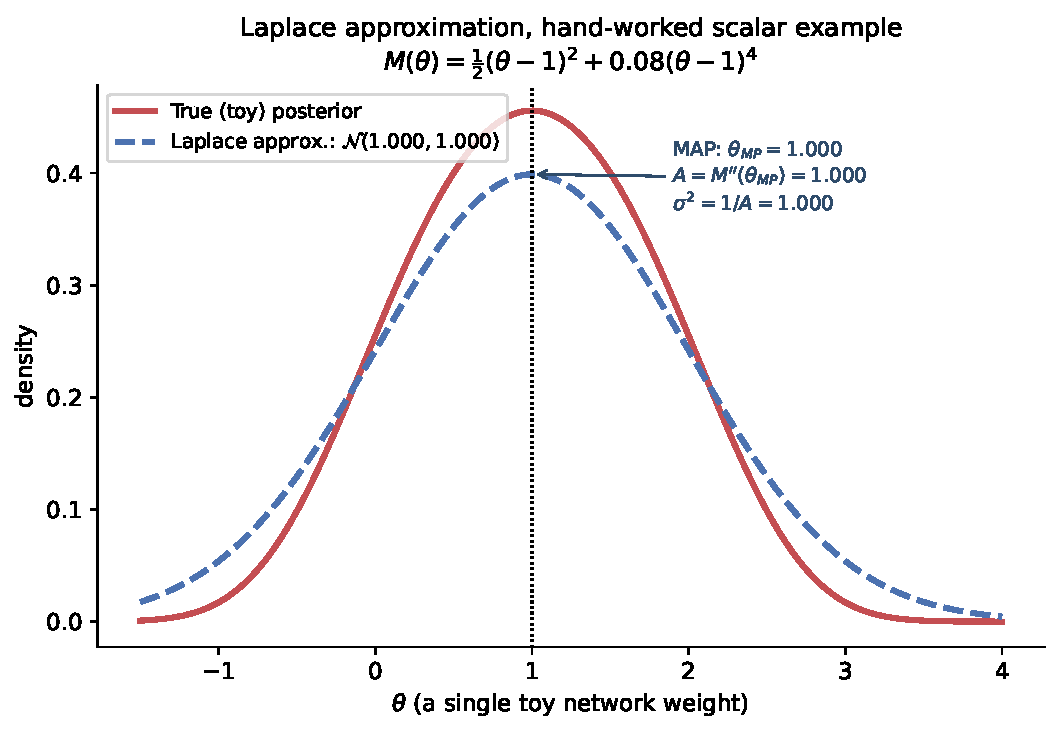
\includegraphics[width=0.72\linewidth]{fig_laplace_1param_toy}
  \end{center}

  The dashed Gaussian is centred exactly at the mode $\theta_{MP}$ and has
  variance $1/A$ where $A = M''(\theta_{MP})$ is the curvature there --
  matching the true posterior's peak height and local width almost
  perfectly, but under-estimating how much probability mass sits in the
  right-hand tail. This is a toy illustration of the exact same trade-off
  that MacKay's Laplace approximation makes for full neural networks with
  hundreds of parameters.

\end{frame}

\begin{frame}[fragile]{Python: Laplace Approximation Step by Step (Toy Example)}

The code below performs the four Laplace-approximation steps on a tiny toy
network by hand: find the MAP estimate by minimising the penalised loss,
numerically approximate the Hessian at that point, invert it to get the
posterior covariance, and use the resulting Gaussian to get a predictive
standard deviation. This mirrors exactly what a library such as
\texttt{laplace-torch} automates for a full-sized network.

\begin{lstlisting}[caption={MAP, Hessian, and predictive uncertainty by hand}]
import numpy as np
from scipy.optimize import minimize

def neg_log_posterior(theta, x, y, alpha, beta, forward):
    # M(w) = alpha*E_w + beta*E_D  (Eq. 10.6)
    resid = y - forward(theta, x)
    return 0.5*alpha*np.sum(theta**2) + 0.5*beta*np.sum(resid**2)

# Step 1: find w_MP by minimising M(w) -- ordinary MAP training
result = minimize(neg_log_posterior, theta0,
                   args=(x_train, y_train, alpha, beta, forward),
                   method="BFGS", jac=grad_neg_log_posterior)
theta_map = result.x

# Step 2: numerically approximate the Hessian A at theta_map
#         (finite-difference the analytic gradient)
A = numerical_hessian(theta_map, x_train, y_train, alpha, beta)

# Step 3: posterior covariance = inverse Hessian  (Eq. 10.7-10.8)
Sigma = np.linalg.inv(A)

# Step 4: propagate uncertainty to a new input x_star via the
#         delta method:  Var[f(x_star)] ~= J(x_star) . Sigma . J(x_star)^T
J_star = jacobian(theta_map, x_star)
pred_mean = forward(theta_map, x_star)
pred_var  = J_star @ Sigma @ J_star
pred_std  = np.sqrt(pred_var + 1.0/beta)   # + observation noise
\end{lstlisting}

\end{frame}

%% ══════════════════════════════════════════════════════════════════════════
\section{Toy Running Example: A Tiny BNN for Motor Claims}
%% ══════════════════════════════════════════════════════════════════════════

\begin{frame}[allowframebreaks]{A Toy Running Example: Driver Age vs.\ Claim Amount}

To make everything concrete, consider a miniature version of a
motor-insurance-claims regression problem: 6 synthetic (driver age, claim
amount) pairs, loosely mimicking the well-known actuarial pattern that both
very young and older drivers tend to have higher claim costs than
middle-aged drivers (a U-shaped risk profile).

\textbf{This toy dataset and toy network are entirely our own illustrative
simulation, built only to demonstrate the mechanics of Sects.\ 10.2--10.3.
They are not the book's real data or real results -- those are summarised
qualitatively in Sects.\ 10.4--10.5.}

  \begin{exampleblock}{The Toy Data}
    \begin{center}
    \begin{tabular}{lcccccc}
      \toprule
      Driver age (yrs)  & 22  & 28  & 35  & 45  & 55  & 65 \\
      Claim amount (R'000) & 4.8 & 3.1 & 2.0 & 2.4 & 3.4 & 5.1 \\
      \bottomrule
    \end{tabular}
    \end{center}
  \end{exampleblock}

  \begin{block}{The Toy Network}
    We fit a tiny network with two $\tanh$ hidden units plus a linear term:
    \[
      f(x;\bw) = v_1 \tanh(w_1 x + b_1) + v_2 \tanh(w_2 x + b_2) + m x + c,
    \]
    an 8-parameter model ($\bw = (w_1,b_1,v_1,w_2,b_2,v_2,m,c)$), with a
    Gaussian prior of precision $\alpha=0.3$ on every parameter and a
    Gaussian-noise likelihood of precision $\beta=8$ (i.e.\ an assumed
    observation noise standard deviation of $1/\sqrt{8}\approx0.35$, in
    R'000). We follow exactly the four Laplace steps of Sect.\ 10.3.
  \end{block}

  \framebreak

  \begin{block}{Step 1 -- Step 3 Applied to the Toy Data}
    \begin{itemize}
      \item \textbf{Step 1 (MAP):} minimising $M(\bw)$ by gradient-based
        optimisation gives $w_1{=}{-}2.07,\, b_1{=}{-}1.90,\, v_1{=}2.35,\,
        w_2{=}{-}1.19,\, b_2{=}1.02,\, v_2{=}{-}1.04,\, m{=}0.88,\, c{=}5.13$.
        This is exactly what an ordinary (regularised) training run of this
        tiny network would converge to.
      \item \textbf{Step 2 (Hessian):} we numerically approximate the
        $8\times 8$ Hessian $\mathbf{A}$ of $M(\bw)$ at this MAP point by
        central-differencing the analytic gradient. Checking its
        eigenvalues confirms $\mathbf{A}$ is positive definite -- confirming
        this MAP point is a genuine local minimum of the loss (a valid
        prerequisite for the Laplace approximation).
      \item \textbf{Step 3 (posterior covariance):} $\boldsymbol{\Sigma} =
        \mathbf{A}^{-1}$. Some parameters (like $c$, the output bias) end up
        tightly constrained by the data; others (like the input-side hidden
        weights) are left with more residual uncertainty, since only 6 data
        points constrain an 8-parameter model.
    \end{itemize}
  \end{block}

  \begin{block}{Step 4: Propagating Uncertainty to Predictions}
    For any query age $x^*$, the predictive variance is
    $\mathrm{Var}[f(x^*)] \approx \mathbf{J}(x^*)^\top \boldsymbol{\Sigma}\,
    \mathbf{J}(x^*)$, where $\mathbf{J}(x^*)$ is the (analytic) gradient of
    $f(x^*;\bw)$ with respect to every one of the 8 parameters at
    $\bw_{MP}$. The total predictive standard deviation additionally adds the
    observation noise, $\sqrt{\mathrm{Var}[f(x^*)] + 1/\beta}$.
  \end{block}

\end{frame}

\begin{frame}{Toy Result: Predictive Mean and Uncertainty Band}

  \begin{center}
    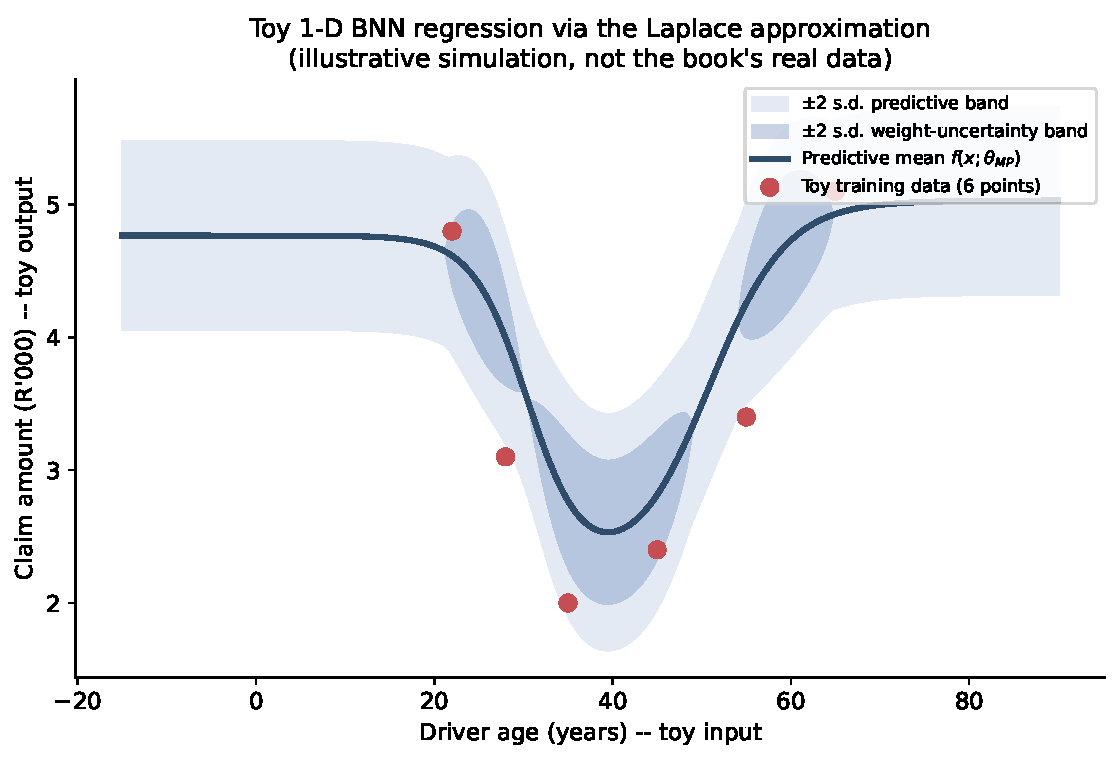
\includegraphics[width=0.75\linewidth]{fig_toy_laplace_1d}
  \end{center}

  \begin{alertblock}{The Key Qualitative Behaviour}
    Near the training ages (22--65 years), the total predictive standard
    deviation stays modest, around $0.45$--$0.60$ (R'000). \textbf{Far
    outside} the training range -- e.g.\ at an extrapolated age of $-15$ or
    $90$ years, deliberately outside anything the network was trained on --
    the standard deviation grows to roughly $2.8$ and $1.8$ (R'000)
    respectively: the band visibly widens. This is exactly the behaviour we
    want from a Bayesian model: it should become \emph{less} confident about
    predictions in regions unlike anything it has seen, precisely the
    opposite of an ordinary point-estimate network, which would output the
    same false confidence everywhere.
  \end{alertblock}

\end{frame}

%% ══════════════════════════════════════════════════════════════════════════
\section{10.4 Numerical Experiments}
%% ══════════════════════════════════════════════════════════════════════════

\begin{frame}[allowframebreaks]{10.4.1 Data Description}

Having built the toy intuition, we return to the book's real numerical
experiments. All numbers in this section and the next are as reported in the
chapter -- not toy numbers.

  \begin{block}{The Dataset}
    3000 records of a non-life motor insurance portfolio from a
    \textbf{Spanish insurance company} (Segura-Gisbert et al., 2024). The
    target variable is \textbf{binary}: whether or not the policy had a
    claim in the given year. Only \textbf{18\% of instances were claims} --
    the dataset is \textbf{highly imbalanced}. All features are normalised
    with a \textbf{min-max scaler} before being used.
  \end{block}

  \begin{block}{The 27 Input Features (Grouped)}
    \begin{columns}[T]
      \column{0.48\textwidth}
        \textbf{Policy administration}: ID, contract start/renewal/next-renewal
        dates, distribution channel (agent vs.\ broker), seniority, policies
        in force, max policies/products ever held, lapse count and date,
        payment method, premium.

        \medskip
        \textbf{Claims behaviour}: \texttt{R\_Claims history} -- the
        proportion of claims relative to total years insured, excluding the
        current year.
      \column{0.48\textwidth}
        \textbf{Driver \& policy risk}: date of birth, driving-licence date,
        type of risk (motorcycle/van/automobile/agricultural), area
        (rural/urban), second driver flag.

        \medskip
        \textbf{Vehicle characteristics}: year of registration, power,
        cylinder capacity, market value, number of doors, fuel type
        (petrol/diesel), length, weight.
    \end{columns}
  \end{block}

  \framebreak

  \begin{block}{Why the ARD Prior on These Features Matters}
    An Automatic Relevance Determination (ARD) prior places a \emph{separate}
    precision hyperparameter on the group of weights entering from each input
    feature. Features that are not useful for prediction get shrunk strongly
    toward zero (their effective weight variance collapses); useful features
    keep meaningful weight variance. This is what allows the chapter to
    \emph{rank} the 27 input features by importance in Sect.\ 10.5, as a
    direct byproduct of Bayesian training -- not a separate post-hoc analysis
    step.
  \end{block}

\end{frame}

\begin{frame}[allowframebreaks]{10.4.2 Experiment Setup and Performance Metrics}

  \begin{block}{Training Setup}
    \begin{itemize}
      \item A \textbf{standard Gaussian} distribution is used as the prior
        for the weights.
      \item The Laplace approximation algorithm is run for \textbf{150
        iterations}.
      \item All computations are performed in Python using the
        \textbf{Laplace PyTorch package} (Daxberger et al., 2021) -- the
        same practical tool introduced conceptually in Sect.\ 10.3.
      \item The \textbf{log evidence} is computed on the training data for
        each of the six architectures (Table 10.1 of Sect.\ 10.2), used for
        model selection: the higher the log evidence, the better the model
        is considered to be, \emph{without} needing to look at held-out
        data.
    \end{itemize}
  \end{block}

  \begin{block}{Performance Metrics on Unseen (Held-Out) Data}
    \begin{itemize}
      \item \textbf{ROC (Receiver Operating Characteristic) curve}: plots
        the true positive rate (correctly flagged claims) against the false
        positive rate (false alarms) as the decision threshold varies.
      \item \textbf{AUC (Area Under the ROC Curve)}: summarises the ROC
        curve in a single number between 0 and 1; measures the average rate
        of correct ranking between a random claim and a random non-claim.
        AUC is particularly well suited here because the correct relative
        cost of a false positive vs.\ a false negative is not known in
        advance -- exactly the situation with this imbalanced (18\% claims)
        dataset.
      \item \textbf{Accuracy}: the overall fraction of correctly classified
        policies on unseen data.
    \end{itemize}
  \end{block}

\end{frame}

\begin{frame}[fragile]{Python: Bayesian Neural Networks via the \texttt{laplace-torch} Package}

This is (schematically) the actual workflow the book uses: train a
point-estimate network exactly as usual, then wrap it with the
\texttt{Laplace} package to obtain the posterior over weights, all without
touching the network's training code.

\begin{lstlisting}[caption={Schematic workflow following Daxberger et al. (2021)}]
import torch, torch.nn as nn
from laplace import Laplace

# 1) Ordinary MAP training: build & train the point-estimate network,
#    e.g. Model 5 -- 2 hidden layers, 10 tanh neurons each (372 params)
model = nn.Sequential(
    nn.Linear(27, 10), nn.Tanh(),
    nn.Linear(10, 10), nn.Tanh(),
    nn.Linear(10, 1),
)
# ... standard training loop with binary cross-entropy loss on
#     whether the policy had a claim ...

# 2) Wrap the trained network with a Laplace approximation
la = Laplace(model, likelihood="classification",
             subset_of_weights="all", hessian_structure="full")
la.fit(train_loader)                 # Step 2: estimate the Hessian A
la.optimize_prior_precision()        # optimise alpha, beta by max evidence

print("Log evidence:", la.log_marginal_likelihood().item())

# 3) Predictive distribution for new policies (mean + uncertainty),
#    obtained by propagating N(w_MP, A^-1) through the network
probs = la(x_new_policies)            # Step 4: predictive distribution
\end{lstlisting}

\end{frame}

%% ══════════════════════════════════════════════════════════════════════════
\section{10.5 Results and Discussions}
%% ══════════════════════════════════════════════════════════════════════════

\begin{frame}[allowframebreaks]{10.5 Results: Model Comparison via the Evidence}

  \begin{block}{Table 10.1 -- Log Evidence, AUC, and Accuracy Across Models}
    \begin{center}
    {\scriptsize
    \begin{tabular}{lcccccc}
      \toprule
      \textbf{Metric} & \textbf{M1} & \textbf{M2} & \textbf{M3} & \textbf{M4} & \textbf{M5} & \textbf{M6} \\
      \midrule
      Parameters   & 137 & 272 & 1352 & 162 & 372 & 472 \\
      Log evidence & $-379.27$ & $-375.75$ & $-390.80$ & $-377.90$ & $\mathbf{-336.27}$ & $-363.50$ \\
      AUC          & 0.7779 & 0.7828 & 0.8035 & 0.7561 & \textbf{0.8407} & 0.7680 \\
      Accuracy     & 0.8908 & 0.8915 & 0.8962 & 0.8915 & \textbf{0.9131} & 0.8938 \\
      \bottomrule
    \end{tabular}
    }
    \end{center}
    \textbf{Model 5} (two hidden layers, 10 neurons each, 372 parameters)
    has both the \textbf{highest log evidence} and the \textbf{best AUC and
    accuracy} on unseen data -- all three metrics agree. Notably, Model 3
    (the largest, with 1352 parameters) has the \emph{worst} log evidence:
    the evidence metric penalises unnecessarily complex models, favouring
    parsimony rather than raw parameter count.
  \end{block}

  \framebreak

  \begin{block}{Table 10.2 -- Pairwise Log Bayes Factors}
    \begin{center}
    {\scriptsize
    \begin{tabular}{lcccccc}
      \toprule
       & \textbf{M1} & \textbf{M2} & \textbf{M3} & \textbf{M4} & \textbf{M5} & \textbf{M6} \\
      \midrule
      M1 & x & 3.51 & $-11.53$ & 1.36 & 42.99 & 15.76 \\
      M2 &   & x & $-15.04$ & $-2.15$ & 39.47 & 12.25 \\
      M3 &   &   & x & 12.89 & 54.52 & 27.30 \\
      M4 &   &   &   & x & 41.63 & 14.40 \\
      M5 &   &   &   &   & x & $-27.22$ \\
      \bottomrule
    \end{tabular}
    }
    \end{center}
    Reading the table: entries compare the column model against the row
    model (e.g.\ the Bayes factor for Model 5 vs.\ Model 2 is 39.47, strongly
    favouring Model 5). \textbf{Model 6 has the highest support against every
    other model except Model 5}, which beats every model including Model 6.
    All pairwise comparisons show a significant difference according to
    Jeffreys' scale for interpreting Bayes factors. The overall pattern:
    \textbf{deeper architectures are preferred to wider-but-shallow ones.}
  \end{block}

\end{frame}

\begin{frame}{Figure 10.2 in the Book: Predictive Performance and Evidence Convergence}

  \begin{exampleblock}{Panel (a): ROC Curves (Described Qualitatively)}
    ROC curves for all six models on unseen data; \textbf{Model 5} sits
    closest to the top-left corner (AUC $= 0.8407$), visibly above the other
    five curves, all of which comfortably beat the ``no skill'' diagonal
    (AUC $=0.5$). The ordering of the curves matches the AUC column of
    Table 10.1 exactly.
  \end{exampleblock}

  \begin{exampleblock}{Panel (b): Marginal-Likelihood Convergence}
    The evidence (marginal likelihood) value plotted across all 150 training
    iterations, for every one of the six models. Every curve flattens out by
    the end of training -- confirming that the Laplace fitting procedure has
    converged for every architecture compared, so the final log-evidence
    values in Table 10.1 are trustworthy for model comparison rather than
    artefacts of early stopping.
  \end{exampleblock}

  \begin{block}{Why This Matters}
    Seeing \emph{both} panels together is important: a model could have high
    AUC purely by chance, or its evidence value could be unreliable if
    training had not converged. Here, the AUC ranking (data-driven, held-out)
    and the evidence ranking (model-driven, computed only on training data)
    agree, and both converge stably -- giving two independent reasons to
    trust Model 5 as the best architecture for this dataset.
  \end{block}

\end{frame}

\begin{frame}[allowframebreaks]{Figure 10.3 and Table 10.3: Which Features Matter Most?}

  \begin{block}{How Feature Importance Falls Out of the ARD Prior}
    Recall from Sect.\ 10.4.1 that the ARD prior gives each input feature its
    own precision hyperparameter. The book's Fig.\ 10.3 plots the
    \textbf{mean posterior variance} of the weights associated with each
    input feature, for every one of the six models: a taller bar means the
    model has left more posterior uncertainty (equivalently, allowed more
    weight magnitude) for that feature, meaning the ARD mechanism judged it
    \emph{more} important, not less.
  \end{block}

  \begin{block}{Table 10.3 -- Top-6 Ranked Features by Model}
    \begin{center}
    {\scriptsize
    \begin{tabular}{lllllll}
      \toprule
      \textbf{Rank} & \textbf{M1} & \textbf{M2} & \textbf{M3} & \textbf{M4} & \textbf{M5} & \textbf{M6} \\
      \midrule
      1 & R Claims hist. & R Claims hist. & R Claims hist. & R Claims hist. & R Claims hist. & R Claims hist. \\
      2 & Type fuel & Type fuel & Policies in force & Type fuel & Type fuel & Date start contract \\
      3 & Lapse & Date next renewal & Lapse & Policies in force & Type risk & Type fuel \\
      4 & Power & Max products & Payment & Max policies & N doors & Cylinder capacity \\
      5 & Date last renewal & Power & Max products & N doors & Cylinder capacity & Policies in force \\
      6 & Max policies & Date last renewal & Date next renewal & Seniority & Lapse & Power \\
      \bottomrule
    \end{tabular}
    }
    \end{center}
  \end{block}

  \begin{alertblock}{The Headline Finding}
    Every single model agrees: \texttt{R\_Claims history} (the policyholder's
    historical claim frequency) is by far the \textbf{single most important
    predictor}, ranked \#1 across all six architectures. This is followed
    consistently by \textbf{vehicle-related features} (fuel type, power,
    cylinder capacity) and by \textbf{how many policies/products} the client
    holds with the insurer -- a broadly consistent, robust picture of what
    drives claim risk in this portfolio.
  \end{alertblock}

\end{frame}

%% ══════════════════════════════════════════════════════════════════════════
\section{10.6 Conclusion}
%% ══════════════════════════════════════════════════════════════════════════

\begin{frame}[allowframebreaks]{10.6 Conclusion}

  \begin{block}{What This Chapter Achieved}
    This chapter presented a \textbf{first-in-literature Bayesian framework}
    for modelling motor insurance claims: Bayesian neural networks with
    Automatic Relevance Determination priors, trained via the \textbf{Laplace
    approximation}. This framework delivers two things simultaneously that a
    point-estimate neural network cannot: (1) a principled way to
    \textbf{select between competing architectures} using the Bayesian
    evidence, and (2) a \textbf{ranking of which input features matter most}
    for the prediction task, as a natural byproduct of the ARD prior.
  \end{block}

  \begin{block}{Key Results}
    \begin{itemize}
      \item The Bayesian evidence metric from the Laplace approximation
        reliably selects the model (Model 5: two hidden layers, 10 neurons
        each) that \emph{also} performs best on held-out AUC and accuracy --
        model selection via evidence and via held-out performance agree.
      \item \textbf{Deeper} network architectures are preferred over
        \textbf{wider-but-shallow} ones for this dataset.
      \item The most critical variable across every architecture is
        \textbf{claim history}, followed by vehicle-related features (fuel
        type, power) and by the number of policies/products the client holds
        with the insurer.
    \end{itemize}
  \end{block}

  \framebreak

  \begin{block}{Limitations and Future Work (as noted in the chapter)}
    \begin{itemize}
      \item The chapter used the Laplace approximation rather than MCMC;
        MCMC methods are guaranteed to converge to the true posterior (given
        enough iterations) and could be explored as an extension, at greater
        computational cost.
      \item The chapter modelled only \emph{whether} a claim occurs (a
        binary classification problem). Future work could instead model the
        \emph{absolute value} of claims, decomposing the problem into claim
        \textbf{frequency} and claim \textbf{severity} -- much closer to how
        actuaries traditionally frame the pricing problem.
    \end{itemize}
  \end{block}

  \begin{alertblock}{Looking Ahead}
    The next chapter turns to a very different application of Bayesian
    computation in quantitative finance: \textbf{shadow and adaptive
    Hamiltonian Monte Carlo methods} are used to calibrate the
    \textbf{Nelson--Siegel yield curve model}, again with the goal of
    obtaining not just point estimates of the calibrated parameters, but full
    uncertainty quantification over both the parameters and the model's
    yield-curve predictions.
  \end{alertblock}

\end{frame}

\end{document}
